%%%%%%%%%%%%%%%%%%%%%%%%%%%%%%%%%%%%%%%%%%%%%%%%%%%%%%%%%%%%%%%%%%%%%%%%%%%%%%
%
% Appendix file included in main project file using \input{}
%
% Assumes that LaTeX2e macros and packages defined in cg_comp.sty are
%   available
%
%%%%%%%%%%%%%%%%%%%%%%%%%%%%%%%%%%%%%%%%%%%%%%%%%%%%%%%%%%%%%%%%%%%%%%%%%%%%%%

 \section{Fretting Model\label{app:fret}}

 \begin{equation}
L^\prime_n = d + \sqrt{\left(X_0 + \Delta N - X_n - d\right)^2 + b^2} \approx X_0 - X_n + \Delta N + \frac{b^2}{2 \left(X_0 + \Delta N - X_n - d\right)}\, ,
 \end{equation}


 \begin{figure}
  \centering
  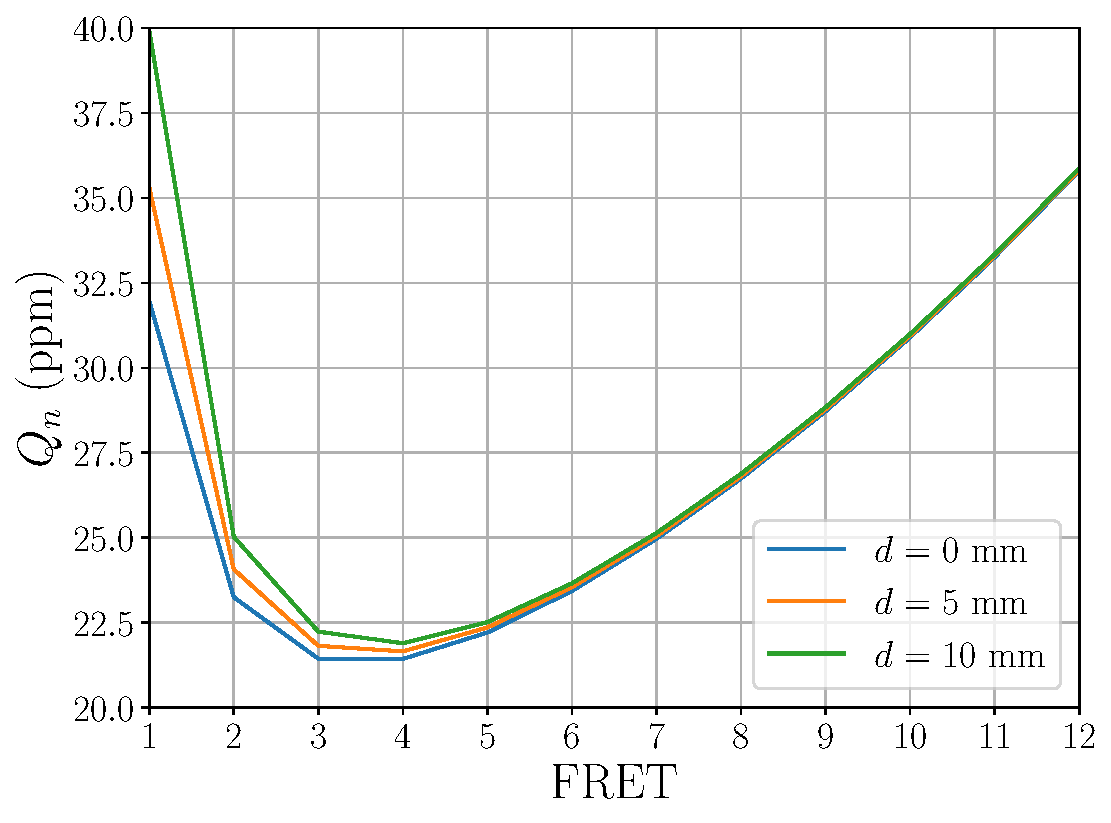
\includegraphics[width=6.0in]{figures/fret_model}
  \caption{\label{fig:fret_model} Plot of the normalized displacement $Q_n$ as a function of the fret number for three different values of the parameter $d$. Here the guitar has $b = 1.0$~mm, $c = 3.5$~mm, no setbacks, and a scale length of 650~mm.}
 \end{figure}



